\documentclass[twoside,twocolumn]{article}

% ------
% Fonts and typesetting settings
\usepackage[english]{babel}
\usepackage[sc]{mathpazo}
\usepackage[T1]{fontenc}
\linespread{1.05} % Palatino needs more space between lines
\usepackage{microtype}
\usepackage{amsmath}
\usepackage{svg}
\usepackage{listings}
\usepackage{tikz}
\usepackage{url}
\usepackage{breakurl}
\usepackage{titlesec}
\usepackage{color}
\usepackage[breaklinks]{hyperref}
\tikzstyle{na} = [baseline=-.5ex]
\usetikzlibrary{shapes,graphs,graphs.standard,quotes,shapes.geometric,arrows,fit,calc,positioning,automata,chains,snakes,decorations.pathreplacing}

% special tikz commands for instruction drawings
\newcommand{\tikzmark}[2]{\tikz[remember picture,baseline=(#1.base)]{\node[inner sep=2pt] (#1) {#2};}}
\tikzset{
    instrtext/.style = {font=\fontsize{25}{22.4}\selectfont},
    instrbit/.style = {font=\fontsize{20}{22.4}\selectfont}
}

%% VHDL listings
\lstdefinelanguage{VHDL}{
   morekeywords={
     library,use,all,entity,is,port,in,out,end,architecture,of,
     begin,and
   },
   morecomment=[l]--
}
\lstdefinestyle{vhdl}{
   language     = VHDL,
   basicstyle   = \ttfamily,
   keywordstyle = \color{keyword}\bfseries,
   commentstyle = \color{comment}
}
\lstset {
    basicstyle=\fontsize{7}{8}\ttfamily
}

%% caption skip
\setlength{\belowcaptionskip}{-5pt}

%% code in text
\newcommand{\code}[1]{\texttt{#1}}

%% page layout
\usepackage[hmarginratio=1:1,top=32mm,bottom=40mm,columnsep=20pt]{geometry}
\usepackage[font=it]{caption}
\usepackage{paralist}
%\usepackage{multicol}

\usepackage{graphicx}


% ------
% Lettrines
\usepackage{lettrine}

% ------
% Abstract
\usepackage{abstract}
	\renewcommand{\abstractnamefont}{\normalfont\bfseries}
	\renewcommand{\abstracttextfont}{\normalfont\small\itshape}

% URL bibtex breaks
\def\UrlBreaks{\do\/\do-\do9}

% ------
% Maketitle metadata
\title{\vspace{-7mm}%
	\fontsize{24pt}{10pt}\selectfont
	\textbf{CCOPI: Implementing a Custom Coprocessor Interface for
    VexRiscv}
	}	
\author{%
	\large
	\textsc{Jens Nazarenus, Dominik Swierzy} \\[2mm]
	\normalsize	RheinMain University of Applied Sciences \\
    \normalsize	\code{\{jens.nazarenus, dominik.swierzy\}@hs-rm.de}
	%\vspace{-5mm}
	}
\date{\today}

\usepackage[utf8]{inputenc}

\usepackage{hyperref}


\begin{document}

\maketitle
%\thispagestyle{fancy}

\begin{abstract}
\noindent This paper introduces CCOPI, a minimal-overhead,
    debug-friendly custom coprocessor interface for the
RISC-V implementation VexRiscv. CCOPI, as well as VexRiscv, is written in
the hardware description language SpinalHDL. The interface is responsible 
for the communication between the coprocessor and the core CPU pipeline of 
VexRiscv and thus helps hardware developers designing  
a coprocessor with a custom instruction-set extension.

CCOPI uses the flexibility of the RISC-V implementation VexRiscv to create 
the interface. This paper also shows how VexRiscv is designed particularly with 
regard to modifications and custom extensions. 
\end{abstract}

\section{Introduction}
Coprocessors in general are used to support the core CPU(s) with the
calculation of specific mathematical operations. A coprocessor aims to
accelerate this specific task over a software implementation of the same
task.

Former coprocessors like the Intel 80387 or Motorolas 68881 were used to
execute IEEE 754 compliant floating point operations and could be
bought as independent components~\cite{motorola, intel198780387}. To use the coprocessors new
instructions were included in the instruction stream of the core CPU.

Nowadays the logic of coprocessors is often included inside the CPU
itself as an instruction-set extension. Well-known examples are the
Intel\textregistered{} x87 
floating point unit (FPU) or the Intel\textregistered{} Advanced Encryption Standard New 
Instructions (AES-NI)~\cite{x87, aesni}. Both modules introduce new
instructions, which can
be used by developers.
CCOPI is designed to produce coprocessors which resides inside the core
RISC-V CPU, named VexRiscv, similar to x87 or AES-NI discussed above.

Before approaching the main topic CCOPI and its implementation, this paper
gives an introductional overview of RISC-V and the used
hardware description language SpinalHDL.
\section{RISC-V}
RISC-V is the name of an open source instruction-set architecture (ISA),
which has been developed at the University of California,
Berkeley~\cite{riscv}.
The ISA describes the instructions any RISC-V implementation must
implement, plus optional extensions. The required minimum is specified in
the ``Base Integer Instruction Set'' of the User Level ISA.

A RISC-V instruction $instr$ is always encoded in 32 bits.

       \begin{figure}[h]
        \centering
        \resizebox{7.25cm}{!}{
            \begin{tikzpicture}[]
                %% R-type
                \draw[] (0,6) -- (31,6);
                \draw[] (0,7) -- (31, 7);
                \draw[] (0,6) -- (0,7);
                \draw[] (31,6) -- (31,7);

                \draw[] (31-7,6) --(31-7,7);
                \draw[] (31-12,6) --(31-12,7);
                \draw[] (31-15,6) --(31-15,7);
                \draw[] (31-20,6) --(31-20,7);
                \draw[] (31-25,6) --(31-25,7);

                \node[instrtext] at (31-25-3,6.5) {funct7};
                \node[instrtext] at (31-19-3.5,6.5) {rs2};
                \node[instrtext] at (31-15-2.5,6.5) {rs1};
                \node[instrtext] at (31-12-1.5,6.5) {funct3};
                \node[instrtext] at (31-7-2.5,6.5) {rd};
                \node[instrtext] at (31-0-3.5,6.5) {opcode};

                %% bit header
                \node[instrbit] at (0+0.3,7+0.5) {31};
                \node[instrbit] at (31-7-0.3, 7+0.5) {7};
                \node[instrbit] at (31-12-0.5, 7+0.5) {12};
                \node[instrbit] at (31-12+0.5, 7+0.5) {11};
                \node[instrbit] at (31-15-0.5, 7+0.5) {15};
                \node[instrbit] at (31-15+0.5, 7+0.5) {14};
                \node[instrbit] at (31-20+0.5, 7+0.5) {20};
                \node[instrbit] at (31-20-0.5, 7+0.5) {19};
                \node[instrbit] at (31-25+0.5, 7+0.5) {24};
                \node[instrbit] at (31-25-0.5, 7+0.5) {25};
                \node[instrbit] at (31-7+0.3, 7+0.5) {6};
                \node[instrbit] at (31-0.3, 7+0.5) {0};

                %%\node[instrtext] at (33, 6.4) {R-Type};

            \end{tikzpicture}
        }

        \caption[Instruktionstypen]{R-Type instruction format}      
        \label{fig:riscv_r_type}
    \end{figure}

\noindent The notation $instr[fromBit:toBit]$ is used to extract information from
the instruction. Figure \ref*{fig:riscv_r_type} $instr[6:0]$
represents the opcode, which is the identification code for a machine
instruction. Depending on the opcode, $instr[31:7]$ is decoded in
different ways. In Figure \ref*{fig:riscv_r_type} the ``R-Type''
instruction format is shown, which is responsible for Integer-Register-Register
operations, where the operands are located in the registers specified by
$rs1$ and $rs2$. With $instr[11:7]$ the destination register $rd$ is
specified. $funct7$ and $funct3$ define the exact sub operation of the
instruction.

       \begin{figure}[h]
        \centering
        \resizebox{7.25cm}{!}{
            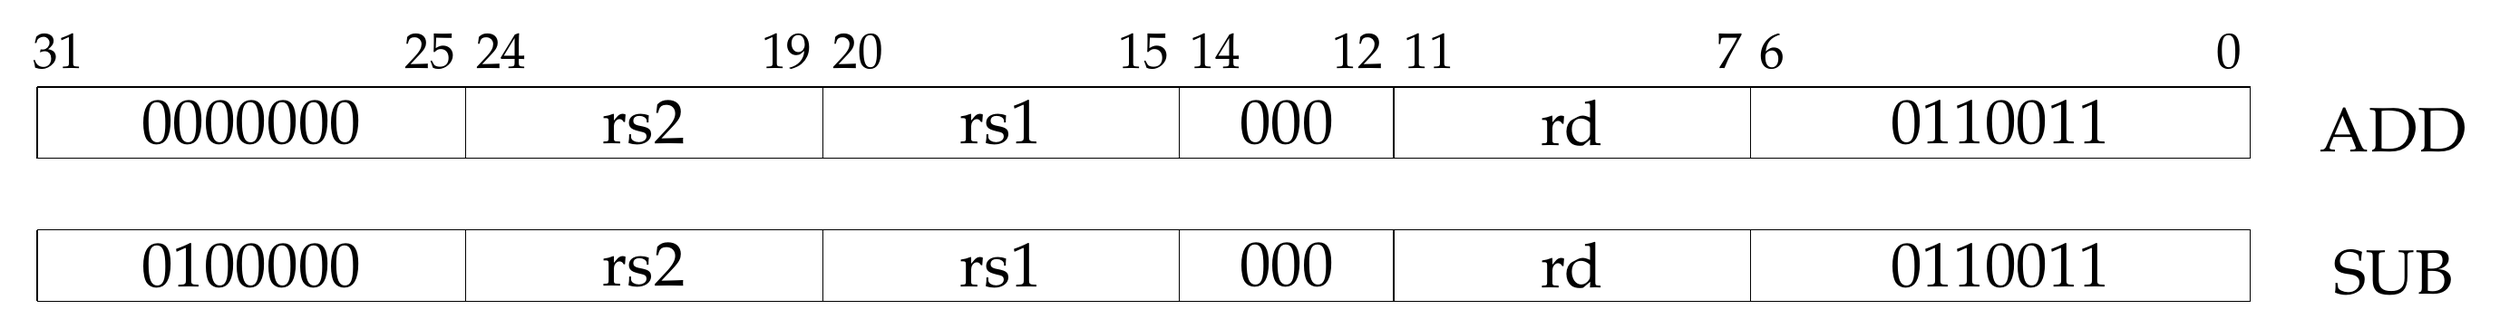
\begin{tikzpicture}[]
                % ADD
                \draw[] (0,6) -- (31,6);
                \draw[] (0,7) -- (31, 7);
                \draw[] (0,6) -- (0,7);
                \draw[] (31,6) -- (31,7);

                \draw[] (31-7,6) --(31-7,7);
                \draw[] (31-12,6) --(31-12,7);
                \draw[] (31-15,6) --(31-15,7);
                \draw[] (31-20,6) --(31-20,7);
                \draw[] (31-25,6) --(31-25,7);

                \node[instrtext] at (31-25-3,6.5) {0000000};
                \node[instrtext] at (31-19-3.5,6.5) {rs2};
                \node[instrtext] at (31-15-2.5,6.5) {rs1};
                \node[instrtext] at (31-12-1.5,6.5) {000};
                \node[instrtext] at (31-7-2.5,6.5) {rd};
                \node[instrtext] at (31-0-3.5,6.5) {0110011};

                % SUB
                \draw[] (0,4) -- (31,4);
                \draw[] (0,5) -- (31, 5);
                \draw[] (0,4) -- (0,5);
                \draw[] (31,4) -- (31,5);

                \draw[] (31-7,4) --(31-7,5);
                \draw[] (31-12,4) --(31-12,5);
                \draw[] (31-15,4) --(31-15,5);
                \draw[] (31-20,4) --(31-20,5);
                \draw[] (31-25,4) --(31-25,5);

                \node[instrtext] at (31-25-3,4.5) {0100000};
                \node[instrtext] at (31-19-3.5,4.5) {rs2};
                \node[instrtext] at (31-15-2.5,4.5) {rs1};
                \node[instrtext] at (31-12-1.5,4.5) {000};
                \node[instrtext] at (31-7-2.5,4.5) {rd};
                \node[instrtext] at (31-0-3.5,4.5) {0110011};


                %% bit header
                \node[instrbit] at (0+0.3,7+0.5) {31};
                \node[instrbit] at (31-7-0.3, 7+0.5) {7};
                \node[instrbit] at (31-12-0.5, 7+0.5) {12};
                \node[instrbit] at (31-12+0.5, 7+0.5) {11};
                \node[instrbit] at (31-15-0.5, 7+0.5) {15};
                \node[instrbit] at (31-15+0.5, 7+0.5) {14};
                \node[instrbit] at (31-20+0.5, 7+0.5) {20};
                \node[instrbit] at (31-20-0.5, 7+0.5) {19};
                \node[instrbit] at (31-25+0.5, 7+0.5) {24};
                \node[instrbit] at (31-25-0.5, 7+0.5) {25};
                \node[instrbit] at (31-7+0.3, 7+0.5) {6};
                \node[instrbit] at (31-0.3, 7+0.5) {0};




                \node[instrtext] at (33, 6.4) {ADD};
                \node[instrtext] at (33, 4.4) {SUB};

            \end{tikzpicture}
        }

        \caption[Instruktionstypen]{ADD, SUB operation}      
        \label{fig:add_sub}
    \end{figure}

\noindent Figure \ref*{fig:add_sub} shows that both, the ADD and the SUB
operation, share the opcode $0110011$. The field $funct7$, which is
decoded in $instr[31:25]$, exposes the exact type of operation:
\begin{itemize}
    \item 0000000 : ADD operation
    \item 0100000 : SUB operation
\end{itemize}
$rs1$, $rs2$ and $rd$ are always encoded at the same positions
in $instr$, to simplify the decoding process in an implementation of
RISC-V~\cite[p. 11]{riscv}.

The ISA also defines opcodes which will not be used by future extensions
and, as a result, available for custom instruction-set extensions~\cite[p.
103]{riscv}:
    \begin{itemize}
        \item $0001011$ : custom-0
        \item $0101011$ : custom-1
        \item $1011011$ : custom-2
        \item $1111011$ : custom-3
    \end{itemize}
The opcodes of custom-2/3 may not be used in RISC-V implementations where the
integer registers are extended to 128 bits (RV128I)~\cite[p. 103]{riscv}. With CCOPI it is
possible to create instruction-set extensions with one or more of the described 
custom opcodes.
\section{SpinalHDL}
The CPU implementation VexRiscv and CCOPI are implemented in the
language ``SpinalHDL'', which is a ``high level hardware description
language'' to describe digital hardware as part of register-transfer
level design~\cite{spinal_doc1}. Output of a compilation process is VHDL or
Verilog code. For this reason SpinalHDL is a transcompiler which takes
Scala code and transforms it into Verilog or VHDL.  

In the following example a component named ``Comp'' is created. The
design adds the two input signals ``a'' and ``b'' with an additional
``x'', which is specified as a Scala class constructor parameter: 
\begin{lstlisting}[language=scala]
class Comp(x: Int) extends Component {
    val io = new Bundle {
        val a, b = in UInt(8 bits)
        val result = out UInt(8 bits)
    }
    io.result := io.a + io.b + x
}
\end{lstlisting}
To generate the module, the compiler of SpinalHDL gets called with one of
the functions \code{SpinalVerilog(component)} or
\code{SpinalVhdl(component)}. The variable ``x'' is set to $15$:
\begin{lstlisting}[language=scala]
object MyComponentGen {
  def main(a: Array[String]): Unit = {
    SpinalVerilog(new Comp(15))
  }
}
\end{lstlisting}
Afterwards the following Verilog code gets emitted in the file
``Comp.v'', where $15$ is resolved to \code{8’b00001111} by the
SpinalHDL compiler:
\begin{lstlisting}[language=verilog]
module Comp (
      input  [7:0] io_a,
      input  [7:0] io_b,
      output [7:0] io_result);
  wire [7:0] zz_1;
  assign zz_1 = (io_a + io_b);
  assign io_result = (zz_1 + 
                     (8'b00001111));
endmodule
\end{lstlisting}
With the combination of Scala and SpinalHDL, it is possible to create
more abstract hardware designs. Object
oriented software patterns like inheritance, polymorphism or type
parametrization are built-in features of Scala and can be used. 
Even higher-order functions like Scalas ``map''
function will get evaluated during the compilation.

The following SpinalHDL code initializes a ROM with predefined values in
a Scala list:
\begin{lstlisting}[language=scala]
def sbox = List(0x63, 0x7C, ...)
val romsbox = Mem(Bits(8 bits), 
                  sbox.map(B(_, 8 bits)))
\end{lstlisting}

\noindent The generated code looks as follows:
\begin{lstlisting}[language=verilog]
module Comp ();
  reg [7:0] romsbox [0:1];
  initial begin
    romsbox[0] = 'b01100011;
    romsbox[1] = 'b01111100;
    ...
  end
endmodule
\end{lstlisting}
SpinalHDL also introduces data types which are divided in composite
types and base types. The available base types are~\cite{spinal_doc2}:
\begin{itemize}
    \item Bool (True, False)
    \item Bits (A vector of Bits, like \code{B"0011"})
    \item UInt/SInt (Unsigned/Signed Integer, used for integer
        arithmetic)
\end{itemize}
Composite types are supposed to group base types. A \code{Bundle} for
example may be used to group the available input/output signals of a
component under a single name:
\begin{lstlisting}[language=scala]
val io = new Bundle {
    val a, b = in UInt(8 bits)
    val result = out UInt(8 bits)
}
\end{lstlisting}
Since SpinalHDL is based on Scala, build tools like SBT can be used to
manage dependencies and compile a SpinalHDL based hardware project. The
dependencies \code{spinalhdl-core} and \code{spinalhdl-lib} are required
to use the language features discussed above:
\begin{lstlisting}[language=scala]
libraryDependencies ++= Seq(
  "com.github.spinalhdl" % "spinalhdl-core_2.11" 
    % "0.10.15",
  "com.github.spinalhdl" % "spinalhdl-lib_2.11" 
    % "0.10.15",
)
\end{lstlisting}

Both, VexRiscv and CCOPI, use the object oriented design pattern paired
with functional programming elements to describe the hardware in an
abstract way. The next chapter gives a more detailed overview of the
RISC-V implementation named VexRiscv.

\section{VexRiscv}
CCOPI uses VexRiscv as its underlying RISC-V implementation. VexRiscv 
implements the ``RV32IM'' instruction set, which means that it contains
the following features~\cite{vexriscv_readme}:
\begin{itemize}
    \item 32 Bit registers
    \item Base Integer instruction set
    \item Standard Extension for Integer
Multiplication and Division
\end{itemize}
The CPU is pipelined on a five-stage RISC pipeline like the MIPS
architecture, whereby the \textbf{Instruction Fetch} stage
copies the next 32-bit instruction in the register ``pc''~\cite[C-34]{computer_architecture}. Once the
instruction is present, the \textbf{Decode} stage analyzes the instruction. 
Based on the opcode,
the Decode stage knows how to interpret $instr[31:7]$ of the
instruction,
which is stored in ``pc''. The \textbf{Execute} stage computes a result
based on the operands which were determined in the Decode stage. One or
more Arithmetic Logical Units (ALU) are used to
perform arithmetic or logical operations in the \textbf{Execute Stage}. 
The \textbf{Memory} stage
handles the Load/Store operations of RISC-V. The final pipeline stage, 
the \textbf{Write Back} stage, copies the result of the Execute stage in
the destination register ``rd'', which is specified in $instr[11:7]$ of
the instruction.
\subsection{Plugin mechanism}
A CPU in general consists of a large number of modules, for example:
\begin{itemize}
    \item Arithmetic Logical Units
    \item Branch prediction module
    \item Pipeline-hazard management module
\end{itemize}
In VexRiscv each module is designed as a \mbox{\textbf{plugin}}, which describes how the
pipeline should behave, when the plugin is active. For this purpose
a module (or plugin) can modify every single pipeline stage. The
compilation process of SpinalHDL resolves the plugins and creates a
pipeline which contains the plugin-specific pipeline
modifications.

A VexRiscv plugin must be programmed against the Trait \code{Plugin}:
\begin{lstlisting}[language=scala]
class SomePlugin extends Plugin[VexRiscv] {

  /** Configure plugin */
  override def setup(p: VexRiscv): Unit = {
  
  }
  
  /** Change pipeline */
  override def build(p: VexRiscv): Unit = {
  
  }
}
\end{lstlisting}
\noindent Once ``\code{extends Plugin[VexRiscv]}'' is defined, the two
functions \code{setup()} and \code{build()} must be implemented. The
configuration of the plugin takes place in the \code{setup()} function.
In the \code{build()} function pipeline modifications can be defined.
For this purpose it is possible to plug into the different pipeline
stanges:
\begin{lstlisting}[language=scala]
override def build(p: VexRiscv): Unit = {
  import pipeline._
  import pipeline.config._

  execute plug new Area {
    // Execute Stage code
  }

  memory plug new Area {
    // Memory Stage code
  }
}
\end{lstlisting}
In the listing above, pipeline specific code can be defined in the
corresponding stage area. With CCOPI, a new instruction-set extension
will be defined in the \code{setup()} function. The communication
between VexRiscv and the coprocessor takes place in the execute- and
memory-stage specific pipeline areas.

\section{CCOPI}
\subsection{Communication}
\label{sec:ccopi-communication}
CCOPI is the name of the custom coprocessor interface for the RISC-V
implementation VexRiscv. It is designed to satisfy the following basic
principles:
\begin{itemize}
    \item A coprocessor is a VexRiscv plugin
    \item A designed coprocessor can also be used without VexRiscv
\end{itemize}
A CCOPI based coprocessor contains one or more ``instruction
functions'', which are hardware operations bound to distinct
instruction patterns. For example a coprocessor named
``SymmetricCryptoCoProcessor'' can be created with the following two
instruction functions:
\begin{itemize}
    \item AES, with the pattern:\\ \code{"-{}-{}-{}-{}-{}-{}-{}-{}-{}-{}-{}-{}-{}-{}-{}-{}-{}000-{}-{}-{}-{}-{}0001011"} 
    \item DES, with the pattern: \\ \code{"-{}-{}-{}-{}-{}-{}-{}-{}-{}-{}-{}-{}-{}-{}-{}-{}-{}001-{}-{}-{}-{}-{}0001011"}
\end{itemize}
Both instruction functions use the custom-0 opcode, but the patterns
differ at $instr[14:12]$ (funct3). The ``-'' signs represent ``Don't-care
bits'' which are not relevant for the decoding process.
\begin{figure}[h]
    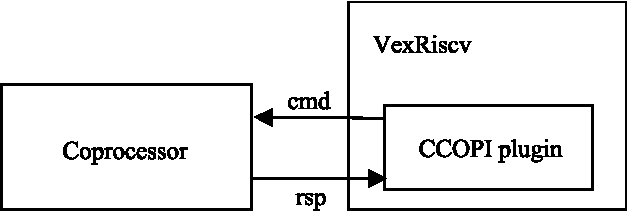
\includegraphics[scale=0.68]{includes/ccopi_plugin}
    \caption{Component structure}
    \label{fig:component_structure}
\end{figure}
\paragraph{Decoder registration.} Since CCOPI is a VexRiscv plugin,
it is possible to register the
instruction patterns at the decoder service of the CPU implementation.
This can be done in the \code{setup()} function of the CCOPI plugin:
\begin{lstlisting}[language=scala]
val decoder = pipeline.service(
                      classOf[DecoderService])
decoder.add(...)
\end{lstlisting}
Once the patterns are registered, the decoder of VexRiscv is able to
decode the instruction functions of CCOPI.



\paragraph{Pipeline modifications.}
Figure \ref*{fig:component_structure} shows that the coprocessor 
is connected with the CCOPI plugin. The communication between them 
is controlled
by a handshake-based protocol named ``Ready/Valid
interface''~\cite{ready_valid}. The
corresponding implementation in SpinalHDL is called ``Stream
bus''~\cite{spinal_doc3}. 

If one of the registered instruction functions gets decoded in the
Decode stage, the CCOPI plugin sends a command (cmd) to the
coprocessor and waits for its response (rsp). To be more precise, the
pipeline gets stalled, until the response is calculated.
\begin{figure}[h]
    \includesvg{includes/ready_valid}
    \caption{Ready/Valid interface example communication for cmd.}
    \label{fig:ready_valid}
\end{figure}

\noindent Figure \ref*{fig:ready_valid} shows the communication of a command,
which is specified in the Execute stage of the CCOPI plugin:
\begin{itemize}
    \item cmd.valid -- set by the CCOPI plugin to indicate that new data
        is available
    \item cmd.payload -- holds the content of the command
    \item cmd.ready -- set by the coprocessor to signal that the data
        transfer is complete
\end{itemize}
The payload of a command is 96 bits wide and contains the following
three 32 bit values:
\begin{itemize}
    \item The current instruction $instr[31:0]$
    \item Register content of rs1, which is specified in $instr[20:15]$
    \item Register content of rs2, which is specified in $instr[24:19]$
\end{itemize}
CCOPI uses inheritance to define the command as SpinalHDL Bundles:
\begin{lstlisting}[language=scala]
class InputBundle extends Bundle {
  val cpuRS1 = Bits(32 bits)
  val cpuRS2 = Bits(32 bits)
}

case class Cmd() extends InputBundle {
  val opcode = Bits(7 bits)
  val rd = Bits(5 bits)
  val tags = Bits(3 bits)
  val rs1 = Bits(5 bits)
  val rs2 = Bits(5 bits)
  val funct = Bits(7 bits)
}
\end{lstlisting}
Note that the Bundle \code{Cmd} represents the introduced R-instruction
type from Figure \ref*{fig:riscv_r_type}. The coprocessor,
however, is not limited to the predefined types, which means
that other interpretations of $instr[31:0]$ are possible.
The response payload is 32 bits wide and will be written to the register
specified in ``rd''.

As an example the emitted Verilog code for a coprocessor with an instruction 
function ``AES'' looks as follows:
\begin{lstlisting}[language=Verilog]
module Coprocessor (
  input aes_comm_cmd_valid,
  output reg aes_communication_cmd_ready,
  input [31:0] aes_comm_cmd_payload_cpuRS1,
  input [31:0] aes_comm_cmd_payload_cpuRS2,
  input [6:0] aes_comm_cmd_payload_opcode,
  input [4:0] aes_comm_cmd_payload_rd,
  input [2:0] aes_comm_cmd_payload_tags,
  input [4:0] aes_comm_cmd_payload_rs1,
  input [4:0] aes_comm_cmd_payload_rs2,
  input [6:0] aes_comm_cmd_payload_funct,
  output aes_comm_rsp_valid,
  input aes_comm_rsp_ready,
  output reg [31:0] aes_comm_rsp_payload_data,
  input clk,
  input reset);

  [...]
endmodule
\end{lstlisting}
The signals, which start with ``\code{aes\_communication\_cmd}'', in
the Verilog code above shortened to ``\code{aes\_comm\_cmd}'', control the
communication from the CCOPI plugin to the coprocessor (command). The
response signals start with the pattern ``\code{aes\_communication\_rsp}''.

In addition, the CCOPI plugin adds the three signals ``\code{\{decode,
execute, memory\}\_cocpu\_aes}'' to the VexRiscv component. These signals are
set to ``high'' when the pipeline executes an instruction for the
coprocessor.

\paragraph{CPU generation.} In SpinalHDL a class, which inherits
\code{Component}, can be used to generate Verilog or VHDL code. In the
CPU implementation the class \code{VexRiscv} must be used for this
purpose. The list of plugins must be passed as a parameter:
\begin{lstlisting}
def cpu() = new VexRiscv(
  config = VexRiscvConfig(plugins = List(
      [...]
      new CoProcessorPlugin(new Cocpu1())
      new CoProcessorPlugin(new Cocpu2())
  ))
)
\end{lstlisting}
The CPU can be generated with the following command and will generate
the file \code{VexRiscv.v}:
\begin{lstlisting}
SpinalVerilog(cpu()) // VexRiscv.v
\end{lstlisting}

\subsection{Coprocessors}
In the previous chapter the plugin mechanism of VexRiscv and the
communication of the CCOPI plugin is described. With CCOPI it is possible
to create coprocessors and instruction functions in an object oriented way.

A coprocessor is a class, which inherits the class
\code{CoProcessor}.
Inside this class it is possible to create instruction functions which are
bound to a specific instruction pattern:
\begin{lstlisting}[language=scala]
def aes = new InstructionFunction[Cmd, Rsp]
          (new Cmd(), new Rsp()) {
  val pattern: String = s"-----------------" +
                         "000-----${custom0}"
  val name: String = "aes"
  val description: String = "AES impl."

  def build(c: EventController): Unit = {
    /** AES implementation */
  }
}

def setup(): Unit = {
  activate(aes)
}
\end{lstlisting}


This code example demonstrates an instruction function named ``aes'', which
is bound to the custom-0 opcode. The function \code{build()} must be
implemented and contains the hardware specific code of the instruction
function, for example the implementation of the symmetric cryptosystem
AES. Each of them must be activated in the \code{setup()} method 
of the coprocessor to indicate SpinalHDL to generate the corresponding
Verilog code.

\begin{table}[h]
\centering
\begin{tabular}{lll}
    Signal name & Type & Mode \\
    \hline
    command & \code{Cmd} & Read-Only \\
    response & \code{Rsp} & Read/Write\\
    done & \code{Bool} & Read-Only\\
    flush & \code{Bool} & Read/Write
\end{tabular}
    \caption{Automatically included signals in \code{build()}}
    \label{tab:signals}
\end{table}
\noindent Table \ref*{tab:signals} shows four signals which get automatically
included in every \code{build()} function. The signal type of
``command''
and ``response'' depends on the definition of
\code{InstructionFunction}. To control the state of the coprocessor,
``done'' and ``flush'' can be used:
\begin{itemize}
    \item done -- false, if the instruction function is busy, true
        otherwise
    \item flush -- User-settable boolean value to signal that the response
        can be transferred to the CPU
\end{itemize}

\subsection{Detailed example}
In the following detailed example a coprocessor named ``ex1'' is
defined. It adds the register content of rs1 and rs2, plus an additional
value of the internal coprocessor ROM. For this purpose five of the
seven most significant bits of the 32 bit instruction can be used to
define the ROM address:
\begin{lstlisting}[language=scala]
class CoProcessorEx1 extends CoProcessor {

  case class Cmd() extends InputBundle {
    val opcode = Bits(7 bits)
    val rd = Bits(5 bits)
    val funct3 = Bits(3 bits)
    val rs1 = Bits(5 bits)
    val rs2 = Bits(5 bits)
    val intRomAddr = Bits(5 bits) // int. RAM
    val funct2 = Bits(2 bits)
  }

  case class Rsp() extends OutputBundle {
    val data = Bits(32 bits)
  }

  def ex1 = new InstructionFunction[Cmd, Rsp]
                (new Cmd(), new Rsp()) {
    val pattern: String = s"00---------------" + 
                           "001-----${custom0}"
    val name: String = "ex1"
    val description: String = "Example 1"

    def build(c: EventController): Unit = {

      val regs = c.prepare event new Area {
        def init = List (0x20, 0x40, 0x60)
        val internalRom = Mem(Bits(8 bits), 
                init.map(B(_ , 8 bits)))
      }

      val exec = c.exec event new Area {
        val counter = Counter(50)

        val romReadAddr = command.intRomAddr
            .asUInt.resize(2)
        val romRead = regs.internalRom
            .readAsync(romReadAddr)
        response.data := (command.cpuRS1.asUInt 
            + command.cpuRS2.asUInt 
            + romRead.asUInt).asBits

        when(counter.willOverflowIfInc) {
          flush := True
        }

        when(!done) {
          counter.increment()
        }.otherwise {
          counter.clear()
        }
      }
    }
  }

  def setup(): Unit = {
    activate(aes)
  }
}
\end{lstlisting}


It is recommended to split the hardware code in two areas:
\begin{itemize}
    \item \code{val x = c.prepare event new Area }
    \item \code{val y = c.exec event new Area }
\end{itemize}
In the ``prepare area'' it is possible to initialize ROMs or define
additional functions. The actual computation should be executed in the 
``exec area''.

In the example above a ROM with three values is initialized in the
``prepare area''. A counter is used in the ``exec area'' to demonstrate
the stalling process of the CPU pipeline. The counter is used to delay the
response flush for 50 cycles.
\paragraph{Usage.}
To use  CCOPI in an Assembler or C application it is necessary to
introduce a new instruction with \code{\#define} statements:

\begin{lstlisting}
#define ccopi_type_insn(_f2, _f5, _rs2, _rs1, \
                        _f3, _rd, _opc) \
.word ( ((_f2)  << 30) | ((_f5)  << 25) | \
        ((_rs2) << 20) | ((_rs1) << 15) | \ 
        ((_f3)  << 12) | ((_rd)  <<  7) | \ 
        ((_opc) << 0))

#define ccopicmd1(_rd, _rs1, _rs2, _iaddr) \
ccopi_type_insn(0b00, _iaddr, _rs2, _rs1, \
                0b001, _rd, 0b0001011)
\end{lstlisting}
The code snippet above defines a new instruction type, where the
most significant seven bits (\code{\_f7}) are split into two 
(\code{\_f2}) and five (\code{\_f5}) bits. In the second \code{\#define}
statement the command \code{ccopicmd1} with the parameters \code{\_rd},
\code{\_rs1}, \code{\_rs2}, and \code{\_iaddr} is introduced.
The internal ROM address of the detailed example can be controlled 
with the \code{\_iaddr} parameter.

\paragraph{Signal naming.} 
A lot of effort has been put into giving the signals reasonable names.
\begin{figure}[h]
    \centering
    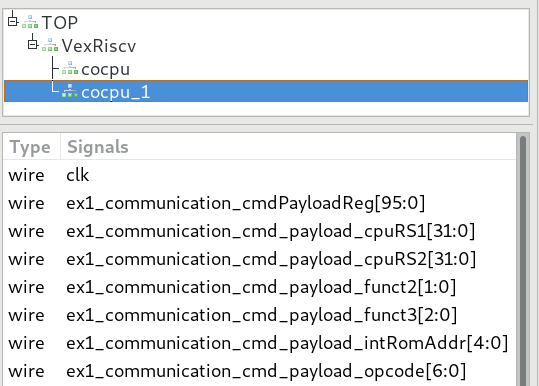
\includegraphics[width=6cm]{includes/gtkwave.png}
    \caption{GTKWave screenshot}
    \label{fig:gtkwave}
\end{figure}

\noindent ``ex1'' is the name of the instruction function in the detailed example
above. For this reason, each signal, which belongs to this specific 
instruction function, starts with ``\code{ex1\_}'', followed by the area 
where the signal is defined:
\begin{itemize}
    \item \code{ex1\_prepare\_<signal-name>}
    \item \code{ex1\_exec\_<signal-name>}
    \item \code{ex1\_communication\_<signal-name>}
\end{itemize}
The last point in the list is the signal pattern, which controls the
internal communication of CCOPI and has already been discussed in
\ref{sec:ccopi-communication}.

Consistent signal names are very helpful for hardware simulation and
debug purposes. Tools like ``Verilator'' use the signal names to
produce a VCD-Trace, which afterwards can be analyzed with a Waveform
viewer like ``GTKWave''. Figure \ref*{fig:gtkwave} shows a GTKWave
screenshot with CCOPI signals. 


\section{Parameters}
Another advantage of CCOPI is the small overhead in terms of 
hardware size and communication latency. Since the size of a result 
computed  by a coprocessor is known before the actual hardware is 
generated, the result can be transferred within one clock cycle via the 
Ready/Valid Interface.

The required number of Lookup tables (LUT) and Flip-Flops for VexRiscv 
depends on the active plugins. For test purposes a minimal configuration 
was chosen, which needs a total of 500 LUTs and 592 Flip-Flops on an 
Artix-7 FPGA. After adding a trivial coprocessor with CCOPI, which 
fills the destination register with zeros, only 34 additional LUTs and 
two more Flip-Flops are needed. This is a rather low price for the huge 
amount of flexibility CCOPI offers.

\section{Future Work}
At the moment CCOPI handles the communication for a synchronous
execution, which means that the CPU pipeline is stalled while the
coprocessor is busy. In the future it should be possible to use
interrupts with the Platform Level Interrupt Controller (PLIC) 
to signal that the result of the coprocessor has been 
determined~\cite{riscv_priv}. With this feature an asynchronous 
execution of one or more coprocessors would be possible. 

\section{Conclusion}
This paper described the implementation of the custom coprocessor
interface CCOPI and its integration in the RISC-V implementation
VexRiscv. SpinalHDL was used as the hardware description language,
which offers the possibility to define high level hardware designs.

CCOPI manages the communication between VexRiscv and a specified
coprocessor automatically. A developer of a coprocessor no longer needs
to worry about the Ready/Valid interface or pipeline stalls. Even in the
leading RISC-V implementation ``Rocket chip'' the communication must be
controlled by the developer,
which makes CCOPI a unique coprocessor interface with a built-in
communication abstraction layer~\cite{rocket-chip_rocc}.

With this in mind it is possible to create a unique
RISC-V CPU with a set of additional functions. As a result, the integration of
existing hardware implementations, like AES, can be achieved in a 
time-efficient way. 

\bibliographystyle{unsrt}
\bibliography{literature}

\end{document}
